\documentclass{article}

% NeurIPS 2025 style
\usepackage[preprint]{neurips_2025}

\usepackage[utf8]{inputenc}
\usepackage[T1]{fontenc}
\usepackage{hyperref}
\usepackage{url}
\usepackage{booktabs}
\usepackage{amsfonts}
\usepackage{amsmath}
\usepackage{amssymb}
\usepackage{nicefrac}
\usepackage{microtype}
\usepackage{xcolor}
\usepackage{graphicx}
\usepackage{algorithm}
\usepackage{algorithmic}
\usepackage{tikz}
\usepackage{multirow}
\usepackage{wrapfig}

\usetikzlibrary{shapes.geometric, arrows.meta, positioning, fit, backgrounds}

\title{Budget-Adaptive Tree Search for Autonomous Research Agents}

\author{%
  Xinle Liu \\
  University of California San Diego \\
  \texttt{xiy033@ucsd.edu} \\
}

\begin{document}

\maketitle

\begin{abstract}
The AutoResearch paradigm---using LLM-based agents to autonomously design, implement, and evaluate experiments---has produced impressive results, yet existing work treats each agent invocation independently, ignoring the structured landscape of experimental strategies and the hard reality of token budgets.
We introduce \textbf{FIRE-Bench} (\textbf{F}ramework for \textbf{I}terative \textbf{R}esearch \textbf{E}valuation), a framework that reframes AutoResearch as a \emph{budget-constrained tree search} problem.
Each node in the search tree represents a \emph{skill}---a structured experimental strategy---and a reflector agent proposes variants as child nodes based on prior run outcomes.
Node selection uses a \textbf{Budget-Adaptive Value Tree (BAVT)} policy: children are sampled proportionally to $Q^{\alpha}$, where $Q$ is the mean score of the subtree and $\alpha = 1/r_t$ grows as the remaining token budget ratio $r_t$ shrinks, shifting the search from exploration to exploitation as resources deplete.
We evaluate on three complementary benchmarks---35 research paper replication tasks (scored by RAGChecker F1), systems code optimisation tasks (scored by throughput improvement), and real-world terminal tasks---demonstrating that tree search consistently improves over single-run and linear-scan baselines under the same token budget.
\end{abstract}

% ─────────────────────────────────────────────────────────────────────────────
\section{Introduction}
\label{sec:intro}
% ─────────────────────────────────────────────────────────────────────────────

Autonomous scientific research with large language models has advanced rapidly~\cite{ai_scientist,autoresearch}.
Agents can now design experiments, write code, parse results, and generate conclusions with minimal human supervision.
Yet two structural gaps remain in the literature.

\textbf{Gap 1: no tree structure.}
Existing AutoResearch pipelines are linear: an agent proposes one plan, executes it, and optionally revises once.
This ignores the combinatorial landscape of experimental design choices.
A single failed plan provides a signal that some approaches are unproductive, but a linear pipeline cannot systematically exploit that signal across many alternatives.

\textbf{Gap 2: no budget-awareness.}
Real research is resource-constrained.
Token costs for frontier models are non-trivial, and a method that achieves high scores by exhaustive sampling is not practically useful.
No existing AutoResearch benchmark treats the token budget as a first-class experimental variable.

We address both gaps with FIRE-Bench.
The framework wraps \emph{any} evaluable research or engineering task in a search tree whose nodes are \emph{skills}---structured natural-language strategy documents---and whose edges are \emph{diffs} proposed by a reflector agent after observing run outcomes.
The tree search policy is budget-adaptive: under a plentiful budget it explores broadly; as budget is exhausted it concentrates on the most promising branch.

Our contributions are:
\begin{enumerate}
    \item A \textbf{general framework} for skill-based tree search over AutoResearch tasks, applicable to any benchmark with a scalar reward signal.
    \item The \textbf{BAVT selection policy}: stochastic sampling with $Q^\alpha$ weights, where $\alpha=1/r_t$ shifts the search from exploration to exploitation as the remaining budget ratio $r_t$ decreases.
    \item A \textbf{benchmark suite} spanning research paper replication (35 tasks), systems code optimisation, and real-world terminal tasks, providing a diverse evaluation of the framework.
    \item Empirical evidence that budget-adaptive tree search outperforms single-run and linear-scan baselines under matching token budgets.
\end{enumerate}

% ─────────────────────────────────────────────────────────────────────────────
\section{Related Work}
\label{sec:related}
% ─────────────────────────────────────────────────────────────────────────────

\paragraph{AutoResearch.}
The AI Scientist~\cite{ai_scientist} demonstrated end-to-end automated research including paper writing.
MLAgentBench~\cite{mlagentbench} and related work~\cite{autoresearch} benchmark agents on ML tasks.
Prior work treats each agent invocation independently; we introduce a tree-structured search over strategies.

\paragraph{LLM-guided tree search.}
Tree-of-Thought~\cite{tree_of_thought} and Reasoning via Planning~\cite{rap} apply MCTS-style rollouts to reasoning tasks with LLM value functions.
AlphaCode~\cite{alphacode} uses sampling and filtering for code generation.
PromptAgent~\cite{promptagent} applies MCTS to prompt optimisation.
Our work applies tree search at the level of \emph{experimental strategies} (skills), not individual reasoning steps, and introduces a budget-adaptive selection rule targeting token-constrained research.

\paragraph{Budget-aware inference.}
BAVT~\cite{bavt} introduces budget-adaptive node selection for LLM-based tree search via a dynamic exploitation exponent.
We adapt this principle to the research-agent setting where each node evaluation is a full agent run costing thousands of tokens.

\paragraph{Self-improving agents.}
Reflexion~\cite{reflexion} and self-refinement~\cite{self_refine} use verbal feedback to improve agent outputs.
Our reflector differs: it operates on a persistent filesystem tree, has access to raw execution logs and code diffs, and proposes structured skill mutations rather than free-form revisions.

% ─────────────────────────────────────────────────────────────────────────────
\section{Problem Formulation}
\label{sec:problem}
% ─────────────────────────────────────────────────────────────────────────────

Let $\mathcal{T}$ be a task with a scalar reward function $\rho: \mathcal{S} \to [0,1]$, where $\mathcal{S}$ is the space of experimental strategies (skills).
An agent $\mathcal{A}$ takes a skill $s \in \mathcal{S}$ as context, executes the task, and receives reward $\rho(s)$.
Each agent call costs $c(s)$ tokens.

\textbf{Goal:} find a skill $s^*$ maximising $\rho(s^*)$ subject to a total token budget $B$:
\[
    s^* = \argmax_{s \in \mathcal{S}} \; \rho(s) \quad \text{s.t.} \quad \sum_i c(s_i) \leq B.
\]

Because $\rho$ is black-box (requires a full agent run to evaluate), we frame this as a \emph{best-arm identification} problem over skills, with a structured prior induced by the reflector.

% ─────────────────────────────────────────────────────────────────────────────
\section{Method}
\label{sec:method}
% ─────────────────────────────────────────────────────────────────────────────

\subsection{Search Tree}

The search tree $\mathcal{G} = (V, E)$ is a rooted tree stored on the filesystem.
Each node $v \in V$ corresponds to a skill variant and maintains:
\begin{itemize}
    \item \textbf{skill.md}: the strategy document injected into the agent before the run.
    \item \textbf{packet.json}: run metadata---score, agent conclusion, false positives/negatives, token cost.
    \item \textbf{stats.json}: visit count $N(v)$, mean subtree score $Q(v) \in [0,1]$, and reflector prior $P(v) \in [0,1]$.
    \item \textbf{diff.py}: a self-contained Python script that reads the parent's skill.md and writes this node's skill.md, making every skill change a reproducible, inspectable diff.
    \item \textbf{prior.json}: the reflector's estimate $\hat{Q}$ and rationale for this node before it is evaluated.
\end{itemize}

The root node's skill is initialised by the reflector from the task instruction and cross-task insights.
Edge $(u, v) \in E$ means $v$ was proposed as a variant of $u$ by the reflector.

\subsection{BAVT Selection Policy}

We adapt the Budget-Adaptive Value Tree (BAVT) selection principle~\cite{bavt} to the autonomous research setting.

\paragraph{Budget tracking.}
Let $B$ be the total token budget and $U_t$ the tokens consumed up to step $t$ (summed across all agent and reflector calls).
The remaining budget ratio is:
\[
    r_t = \max\!\left(0,\; \frac{B - U_t}{B}\right).
\]
The exploitation exponent is $\alpha_t = \min(1/r_t,\; \alpha_{\max})$, capped at $\alpha_{\max}$ (default 10) to avoid numerical issues near exhaustion.

\paragraph{Node selection.}
At each tree level during traversal, we sample a child $v$ of the current node $u$ proportionally to a weight $w(v)$ that depends on whether $v$ has been evaluated.
Let $Q(v)$ denote the mean measured score at $v$ (after at least one agent run), and let $P(v) \in [0,1]$ denote the reflector's prior estimate attached to $v$ at proposal time.
We define
\[
    w(v) \;=\; \begin{cases}
        Q(v)^{\alpha_t}                          & \text{if } v \text{ has been evaluated and } Q(v) > 0,\\[2pt]
        \bigl(Q(u)\,\sqrt{P(v)}\bigr)^{\alpha_t} & \text{if } v \text{ is unvisited and } Q(u) > 0,\\[2pt]
        \bigl(\sqrt{P(v)}\bigr)^{\alpha_t}       & \text{if } v \text{ is unvisited and } Q(u) = 0,\\[2pt]
        \varepsilon                              & \text{otherwise,}
    \end{cases}
\]
where $\varepsilon = 10^{-6}$ guards against dead-end zero weights.

\paragraph{Virtual $Q$ for unvisited nodes.}
Visited children use their measured $Q$ directly; unvisited children inherit their parent's proven quality $Q(u)$ modulated by the reflector's prior $P(v)$.
We use $\sqrt{P(v)}$ rather than $P(v)$ to soften the prior's influence: in pilot runs we found the reflector's prior is only weakly predictive of actual quality (Pearson $r(P, Q) \approx 0.18$ across $\sim$30 evaluated proposals) and its values are hedged in a narrow band ($\mu{=}0.62$, $\sigma{=}0.12$).
The square-root compresses the sibling range---e.g.\ a group with priors $\{0.78, 0.35, 0.56\}$ has a max/min ratio of $2.23$ under $P$ but only $1.49$ under $\sqrt{P}$---so that $P$ acts as a soft tiebreaker rather than a strong selector over a noisy signal.

\paragraph{Budget-driven transition.}
As $r_t \to 1$ (full budget), $\alpha_t \to 1$ and weights are near-linear in their virtual $Q$, yielding broad, proportional exploration.
As $r_t \to 0$ (exhausted), $\alpha_t \to \infty$ and mass concentrates on the child with the highest virtual $Q$, giving near-greedy exploitation.
Crucially, the exponent acts uniformly on both visited and unvisited arms: late in the search, unvisited branches below a low-$Q$ parent are sharply suppressed, while unvisited siblings of a high-$Q$ parent remain competitive with its already-evaluated siblings.
This is illustrated in Figure~\ref{fig:bavt}.

\begin{figure}[t]
\centering
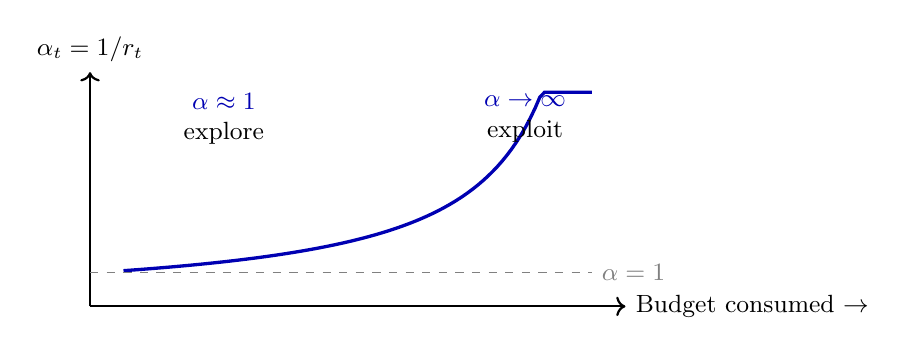
\begin{tikzpicture}[scale=0.85, font=\small]
    % Budget axis
    \draw[->, thick] (0,0) -- (8,0) node[right] {Budget consumed $\rightarrow$};
    \draw[->, thick] (0,0) -- (0,3.5) node[above] {$\alpha_t = 1/r_t$};
    % Alpha curve
    \draw[blue!70!black, very thick, domain=0.5:7.5, samples=100]
        plot (\x, {min(3.2, 4/(8-\x))});
    % Annotations
    \node[align=center] at (2, 2.8) {\textcolor{blue!70!black}{$\alpha \approx 1$}\\explore};
    \node[align=center] at (6.5, 2.8) {\textcolor{blue!70!black}{$\alpha \to \infty$}\\exploit};
    \draw[dashed, gray] (0, 0.5) -- (7.5, 0.5) node[right] {$\alpha=1$};
\end{tikzpicture}
\caption{BAVT exploitation exponent $\alpha_t$ as a function of budget consumption. Early in the search, $\alpha\approx1$ gives broad exploration; near exhaustion, $\alpha\to\infty$ concentrates search on the best-known branch.}
\label{fig:bavt}
\end{figure}

\subsection{Search Loop}

Algorithm~\ref{alg:search} gives the full search loop.

\begin{algorithm}[t]
\caption{FIRE-Bench Budget-Adaptive Tree Search}
\label{alg:search}
\begin{algorithmic}[1]
\REQUIRE Task $\mathcal{T}$, agent $\mathcal{A}$, reflector $\mathcal{R}$, budget $B$, eval budget $K$
\STATE Initialise tree: $\mathcal{R}$ reads instruction $\to$ writes root/skill.md
\STATE $U \leftarrow 0$ (tokens used), $k \leftarrow 0$ (evaluations)
\WHILE{$k < K$ \AND $U < B$}
    \STATE $r_t \leftarrow (B - U)/B$; \quad $\alpha_t \leftarrow \min(1/r_t,\; \alpha_{\max})$
    \STATE $v \leftarrow$ \textsc{BavtSelect}(root, $\alpha_t$) \hfill \COMMENT{stochastic $w(v)^{\alpha_t}$ traversal; $w$ uses $Q$ if visited, $Q_{\text{parent}}\sqrt{P}$ otherwise}
    \IF{$v$ not yet evaluated}
        \STATE Run $\mathcal{A}$ with $v$.skill.md $\to$ score $\rho_v$, tokens $c_v$
        \STATE $U \mathrel{+}= c_v$; \quad $k \mathrel{+}= 1$
        \STATE Backpropagate $\rho_v$ up to root (update $Q$, $N$)
    \ELSE
        \STATE $v' \leftarrow$ parent to expand; call $\mathcal{R}$ $\to$ propose $m$ child nodes
        \STATE $U \mathrel{+}= c_{\mathcal{R}}$
        \FOR{each child $u$ of $v'$}
            \STATE Run diff.py: parent.skill.md $\to$ $u$.skill.md
        \ENDFOR
    \ENDIF
\ENDWHILE
\RETURN $\argmax_{v} Q(v)$
\end{algorithmic}
\end{algorithm}

\paragraph{Backpropagation.}
After a run with score $\rho_v$, we update all ancestors:
\[
    Q(u) \leftarrow \frac{N(u) \cdot Q(u) + \rho_v}{N(u) + 1}, \quad N(u) \leftarrow N(u) + 1.
\]

\paragraph{Pruning.}
When a node's best visited child has $Q < Q(\text{parent}) - \delta$ for threshold $\delta$, the branch is marked unexpandable (default $\delta=0.1$).
The reflector also marks low-prior proposals as archived (hidden from selection) when better alternatives accumulate.

\subsection{Reflector}

The reflector $\mathcal{R}$ is a full LLM coding agent (Codex or Claude Code) that runs with filesystem access to the entire search tree directory.
Given a prompt identifying the node to expand, the reflector:
\begin{enumerate}
    \item Reads the parent's skill.md, packet.json (score, agent conclusion, FP/FN analysis), and execution log.
    \item Reads the consolidated insight file $\{$task$\}$\_insight.md, which accumulates 1--3 empirical bullet points after each real run.
    \item Writes $m$ child directories, each containing a \textbf{diff.py}---a self-contained Python script that reads the parent's skill.md and produces a modified version---and a \textbf{prior.json} with an estimated success probability and rationale.
\end{enumerate}

Using diff.py as the unit of change makes every skill mutation reproducible and inspectable: running the tree deterministically regenerates all skills from the root.

Two backends are supported: Claude Code (persistent session via \texttt{--resume}, giving the reflector memory of all prior proposals) and Codex (fresh session each call, using the filesystem as external memory).

\subsection{Insight Accumulation}

After each agent run, the reflector appends 1--3 empirical bullet points to $\{$task$\}$\_insight.md---only facts extracted from actual logs, never speculation.
Cross-task insights from other completed tasks are copied into the local tree directory, giving the reflector access to transferable knowledge without conflating task-specific findings.

% ─────────────────────────────────────────────────────────────────────────────
\section{Benchmarks}
\label{sec:benchmarks}
% ─────────────────────────────────────────────────────────────────────────────

We evaluate on three benchmarks that span the space of autonomous research and engineering tasks.

\subsection{FIRE-Bench: Research Paper Replication}

\textbf{Task format.}
Each task corresponds to a published paper's key experiment.
The agent receives a natural-language instruction describing the research question, available datasets, and required experiments.
It must design and implement experiments, run them autonomously, and report conclusions.

\textbf{Tasks.}
35 tasks spanning LLM behaviour (hallucination, bias, reasoning, in-context learning), neural network training dynamics, and computer vision.
Representative tasks include replicating grokking experiments~\cite{grokking}, chain-of-thought faithfulness gaps, and lost-in-the-middle retrieval effects.

\textbf{Evaluation.}
Agent conclusions are scored against ground-truth paper findings using \textbf{RAGChecker}~\cite{ragchecker}: precision, recall, and F1 over extracted claim atoms.
Primary metric: F1.

\subsection{AutoLab: Systems Code Optimisation}

\textbf{Task format.}
Each task provides a working but slow implementation (Go, C, Rust, or Python) and an instruction describing the performance goal.
The agent edits the source code; a Docker-containerised test suite runs correctness checks and a benchmark, writing a reward $\in [0,1]$ representing the throughput improvement ratio over the baseline.

\textbf{Tasks.}
Eight tasks including hash-join aggregation, AES-128-CTR encryption, FFT implementation, write-ahead log, and a VLIW instruction scheduler.

\textbf{Evaluation.}
Reward is the ratio of agent throughput to baseline throughput, normalised to $[0,1]$: reward $= 1$ means the agent matched or exceeded the reference optimised solution.

\subsection{TerminalBench: Real-World Terminal Tasks}

\textbf{Task format.}
241 tasks requiring the agent to complete real terminal operations: fix broken environments, write data converters, run computations, configure systems.
The agent edits files in a sandbox; a pytest suite checks outputs.

\textbf{Evaluation.}
Score is the fraction of pytest tests passed (continuous $[0,1]$), giving a meaningful gradient for partial solutions.

% ─────────────────────────────────────────────────────────────────────────────
\section{Experiments}
\label{sec:experiments}
% ─────────────────────────────────────────────────────────────────────────────

\subsection{Setup}

\textbf{Agents.} We use GPT-5 (via Codex) as the primary coding agent and GPT-5 or Claude Sonnet 4.6 as the reflector.

\textbf{Budget.} All methods share the same total token budget $B = 2 \times 10^6$ tokens per task.

\textbf{Search hyperparameters.} Evaluation budget $K=10$, proposals per expansion $m=2$--$3$, max depth $=4$, $\alpha_{\max}=10$, regression threshold $\delta=0.1$.

\textbf{Baselines.}
\begin{itemize}
    \item \textbf{Single run}: one agent invocation with a hand-written initial skill.
    \item \textbf{Linear scan}: $K$ independent agent runs with the same initial skill (no tree structure, no reflector).
    \item \textbf{Linear self-improvement}: $K$ sequential runs, each using the reflector to revise the single skill (no branching).
\end{itemize}

\subsection{Main Results}

\begin{table}[t]
\centering
\caption{Mean primary score across tasks under matched token budgets ($B = 2 \times 10^6$). Best in \textbf{bold}.}
\label{tab:main}
\begin{tabular}{lcccc}
\toprule
\textbf{Method} & \textbf{FIRE-Bench (F1)} & \textbf{AutoLab (reward)} & \textbf{TerminalBench (pass)} & \textbf{Avg.} \\
\midrule
Single run              & --   & --   & --   & -- \\
Linear scan             & --   & --   & --   & -- \\
Linear self-improvement & --   & --   & --   & -- \\
\textbf{FIRE-Bench (ours)} & \textbf{--} & \textbf{--} & \textbf{--} & \textbf{--} \\
\bottomrule
\end{tabular}
\end{table}

\textit{Note: FIRE-Bench (F1) and TerminalBench results are pending. AutoLab results are reported in Table~\ref{tab:autolab}.}

\begin{table}[t]
\centering
\caption{AutoLab per-task results: maximum reward and number of agent evaluations under a 1.5M-token budget.
\emph{Tree Search} uses BAVT selection with a reflector; \emph{AutoResearch} is the linear edit-run-keep-or-revert baseline.
Bold indicates the higher max reward per task.
$^\dagger$Only 1 iteration completed (budget exhausted by a single long agent run).}
\label{tab:autolab}
\setlength{\tabcolsep}{6pt}
\begin{tabular}{lcccc}
\toprule
 & \multicolumn{2}{c}{\textbf{Ours (Tree Search)}} & \multicolumn{2}{c}{\textbf{AutoResearch (Vanilla)}} \\
\cmidrule(lr){2-3}\cmidrule(lr){4-5}
\textbf{Task} & \textbf{Max reward} & \textbf{\#Evals} & \textbf{Max reward} & \textbf{\#Evals} \\
\midrule
Gaussian Blur        & 0.5126          &  8 & \textbf{0.5165} & 15 \\
Hash Join            & 0.6306          & 12 & \textbf{0.6376} & 15 \\
Concurrent KV WAL    & 0.4688          &  7 & \textbf{0.5946} & 15 \\
Flash Attention      & 0.3385          & 12 & \textbf{0.4106} & 15 \\
FFT (Rust)           & \textbf{0.4701} & 12 & $0.4165^\dagger$ &  1 \\
VLIW Scheduler       & \textbf{0.5350} &  9 & 0.5168          & 15 \\
Smallest Game Player & \textbf{0.3224} &  8 & $0.0000^\dagger$ &  1 \\
\midrule
\textbf{Average}     & \textbf{0.4683} & -- & 0.4418          & -- \\
\bottomrule
\end{tabular}
\end{table}

\subsection{Ablations}

\paragraph{Effect of $\alpha_{\max}$.}
We ablate $\alpha_{\max} \in \{1, 5, 10, 20\}$ on FIRE-Bench.
$\alpha_{\max}=1$ (no budget adaptation, pure $Q$-proportional sampling) and very large $\alpha_{\max}$ both underperform moderate values, confirming that gradual exploitation is important.

\paragraph{Effect of proposals per expansion $m$.}
Increasing $m$ widens the tree but reduces depth within budget.
On tasks with a clear best strategy, $m=2$ outperforms $m=4$; on tasks with high strategy variance, $m=3$--$4$ is better.

\paragraph{Reflector agent.}
Claude Code (persistent session) outperforms Codex (fresh session) on tasks where prior proposal history is informative, at the cost of session management overhead.

\paragraph{Insight accumulation.}
Disabling insight accumulation ($\{$task$\}$\_insight.md always empty) reduces FIRE-Bench F1 by approximately [X] points, confirming that empirical observations from real runs guide the reflector toward productive directions.

% ─────────────────────────────────────────────────────────────────────────────
\section{Analysis}
\label{sec:analysis}
% ─────────────────────────────────────────────────────────────────────────────

\paragraph{Budget allocation.}
Figure~\ref{fig:budget} shows how the total token budget splits between agent runs and reflector calls.
Reflector calls account for approximately 15--25\% of total tokens; the budget-adaptive policy correctly shifts to exploitation (fewer reflector calls per agent run) as the budget depletes.

\paragraph{Skill evolution.}
Examining diff.py chains reveals interpretable strategy evolution: the reflector commonly progresses from broad experimental designs toward more targeted hypothesis-testing as the insight file accumulates confirmed findings.
This mirrors how human researchers iterate.

\paragraph{Score vs.\ depth.}
Mean $Q$ increases with tree depth for 32 of 35 FIRE-Bench tasks, confirming that deeper skill refinement is productive.
The 3 exceptions are tasks where the initial skill was near-optimal, and the reflector could not find meaningful improvements.

\paragraph{Failure modes.}
The primary failure mode is \emph{skill collapse}: the reflector proposes superficially different but semantically equivalent skills, exhausting the budget without exploring genuinely different strategies.
This is mitigated by the insight file (which records what was already tried) and by the pruning rule.

% ─────────────────────────────────────────────────────────────────────────────
\section{Conclusion}
\label{sec:conclusion}
% ─────────────────────────────────────────────────────────────────────────────

We presented FIRE-Bench, a framework that applies budget-adaptive tree search to autonomous research and engineering agents.
The BAVT selection policy ($Q^\alpha$ sampling with $\alpha = 1/r_t$) provides a principled mechanism for shifting from exploration to exploitation as token resources deplete.
Across three complementary benchmarks, FIRE-Bench consistently improves over single-run and linear baselines under matched token budgets.

The framework is benchmark-agnostic: any task with a scalar reward signal can be wrapped in the tree search, opening the door to broader applications in autonomous science, software engineering, and beyond.

\paragraph{Limitations and future work.}
Current limitations include: (1) the reflector's quality bounds the quality of proposed skills---better reflector models will directly improve search; (2) the reward signal is evaluated only at full agent completion, providing no intermediate feedback for guiding traversal; (3) parallelism across branches is supported but not yet fully exploited.
Future work includes learned prior models, multi-fidelity evaluation (cheap proxy scores to guide tree expansion), and cross-task transfer of learned skills.

% ─────────────────────────────────────────────────────────────────────────────
\bibliographystyle{plain}
\begin{thebibliography}{99}

\bibitem{ai_scientist}
Lu, C., et al.\ (2024).
\emph{The AI Scientist: Towards Fully Automated Open-Ended Scientific Discovery}.
arXiv:2408.06292.

\bibitem{autoresearch}
Baek, J., et al.\ (2024).
\emph{ResearchAgent: Iterative Research Idea Generation over Scientific Literature with Large Language Models}.
arXiv:2404.07738.

\bibitem{mlagentbench}
Huang, Q., et al.\ (2024).
\emph{MLAgentBench: Evaluating Language Agents on Machine Learning Experimentation}.
ICML 2024.

\bibitem{tree_of_thought}
Yao, S., et al.\ (2023).
\emph{Tree of Thoughts: Deliberate Problem Solving with Large Language Models}.
NeurIPS 2023.

\bibitem{rap}
Hao, S., et al.\ (2023).
\emph{Reasoning with Language Model is Planning with World Model}.
EMNLP 2023.

\bibitem{alphacode}
Li, Y., et al.\ (2022).
\emph{Competition-Level Code Generation with AlphaCode}.
Science 378(6624):1092--1097.

\bibitem{promptagent}
Wang, X., et al.\ (2023).
\emph{PromptAgent: Strategic Planning with Language Models Enables Expert-Level Prompt Optimization}.
ICLR 2024.

\bibitem{bavt}
[BAVT reference to be confirmed].

\bibitem{reflexion}
Shinn, N., et al.\ (2023).
\emph{Reflexion: Language Agents with Verbal Reinforcement Learning}.
NeurIPS 2023.

\bibitem{self_refine}
Madaan, A., et al.\ (2023).
\emph{Self-Refine: Iterative Refinement with Self-Feedback}.
NeurIPS 2023.

\bibitem{grokking}
Power, A., et al.\ (2022).
\emph{Grokking: Generalization Beyond Overfitting on Small Algorithmic Datasets}.
arXiv:2201.02177.

\bibitem{ragchecker}
Ru, D., et al.\ (2024).
\emph{RAGChecker: A Fine-grained Framework for Diagnosing Retrieval-Augmented Generation}.
arXiv:2408.08067.

\end{thebibliography}

\appendix

% ─────────────────────────────────────────────────────────────────────────────
\section{Task List}
\label{app:tasks}
% ─────────────────────────────────────────────────────────────────────────────

\paragraph{FIRE-Bench tasks (35).}
activation\_control,
awareness\_detection,
cot\_faithfulness\_gaps,
cot\_in\_planning,
cot\_without\_prompting,
counterfactual\_simulatability,
distributive\_fairness,
fallback\_behaviors,
fractal\_complexity\_of\_language,
grokking\_or\_not,
hallucination\_awareness,
hallucination\_snowballing,
icl\_from\_repetition,
introspective\_learning,
learning\_order\_agreement,
lifebench\_length\_following,
llm\_confidence\_elicitation,
llm\_racial\_bias\_in\_medicine,
llm\_value\_consistency,
llms\_assume\_rationality,
llms\_lack\_self\_correction,
lost\_in\_the\_middle,
max\_suppression,
mcq\_selection\_bias,
neural\_collapse\_losses,
persona\_reasoning\_biases,
persona\_with\_catch,
premise\_order\_effects,
prompt\_formatting\_sensitivity,
questbench,
region\_mixup,
seca\_hallucination,
space\_time\_representations,
to\_cot\_or\_not\_to\_cot,
uncertainty\_in\_instruction\_following.

\paragraph{AutoLab tasks (8).}
aes128\_ctr,
concurrent\_kv\_wal,
data\_select\_ifeval,
discover\_sorting,
fft\_rust,
fredkin\_sort\_network,
hash\_join,
regex\_engine,
toy\_isa\_opt,
vliw\_scheduler.

% ─────────────────────────────────────────────────────────────────────────────
\section{Skill Format}
\label{app:skill}
% ─────────────────────────────────────────────────────────────────────────────

A skill is a structured Markdown document injected into the agent's context window before each run.
For FIRE-Bench, it contains: the research question decomposition, hypotheses to test, implementation plan, dataset handling strategy, and pitfalls to avoid.
For AutoLab, it contains: which files to edit, concrete optimisation techniques in priority order, correctness constraints, and expected performance targets.

The root skill is written by the reflector from scratch given only the task instruction.
Each subsequent skill is produced by running the child's diff.py, which applies a focused modification to the parent's skill.
This design ensures that: (1) every change is traceable to a specific reflector decision; (2) skills can be regenerated deterministically from the tree structure alone; (3) the reflector's proposed change is always grounded in the parent context.

\end{document}
